\section{RNN}
Una TS è una \textbf{sequenza} di dati dispegata nel tempo. I dati sono tra loro correlati, quindi per una classica rete neurale bisognerebbe creare un input layer di dimensione pari alla lunghezza della TS in modo tale che la rete si alleni su una time series alla volta.\\
Essendo che le TS non sono quasi mai tutte della stessa lunghezza, bisognerebbe definire una rete differente per ogni tipologie di TS. Inoltre, l'input layer crescerebbe troppo.\\
\\
Un'idea potrebbe essere quella di lanciare diverse istanze della medesima rete neurale affinché ciascuna operi su porzioni diverse della serie, per poi mettere insieme i risultati, riprendendo un po' l'idea di un ensemble. \\
Questa soluzione, per quanto semplice, non funziona bene con sequenze di dati, poiché i dati sono tra loro correlati nel tempo: ogni valore nel tempo $t$ è legato al valore nel tempo $t-1$. Con questa soluzione le reti si addestrano su sottosequenze indipendenti della stessa TS, perdendo le correlazioni esistenti.\\
\\
Una \textbf{rete neurale ricorrente} (Recurrent Neural Network, RNN) è in grado di tenere memoria della sottosequenza analizzata nel passato e di prendere decisioni in funzione di esse.\\
Una RNN usa l'output del layer ricorrente come input dello stesso per certo numero di volte. Tra una ripetizione e l'altra i pesi calcolati dall'algoritmo di training sono conservati, così da tenere la memoria della sottosequenza di dati visti precedentemente.\\
I pesi che evolvono nel tempo formano il cosiddetto \textit{hidden state}. Questa tecnica viene chiamata \textbf{parameter sharing}.\\
La dimensione del layer ricorrente è fissata e andrà a determinare, chiaramente, le dimensioni dell'input e dell'output, e corrisponderà alla dimensione della sottosequenza che si desidera analizzare ad ogni passo.
\begin{figure}[H]
	\centering
	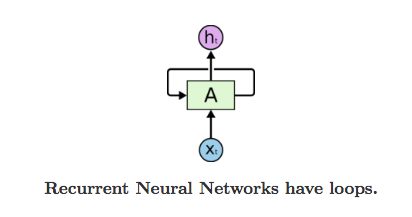
\includegraphics[width=\linewidth]{rnn.png}
	\caption{L'architettura base di una RNN}
	\label{fig:rnn}
\end{figure}
E' molto comune dare una rappresentazione \textit{unrolled} della rete per poterla ricondurre ad una rete neurale classica e comprenderne il funzionamento nel dettaglio.
\begin{figure}[H]
	\centering
	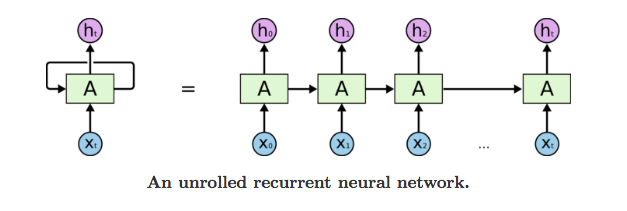
\includegraphics[width=\linewidth]{rnn_unrolled.png}
	\caption{La rappresentazione unrolled di una RNN}
	\label{fig:rnn_unrolled}
\end{figure}
Chiaramente, è possibile rendere più profonda una RNN, ed esistono diversi modi per farlo:
\begin{itemize}
	\item Aggiungere dei layer nascosti ricorrenti. Detta soluzione \textbf{stacked};
	\item Rendere il layer ricorrente una sotto-rete profonda;
	\item Aggiungere dei layer tra l'input e quello ricorrente;
	\item Aggiungere dei layer tra il ricorrente e l'output;
\end{itemize}

\subsection{LSTM}
Come evidenziato da bengio et al.\cite{long_term}, il modello standard di RNN nella pratica soffre di un problema long-term dependencies. Man mano che la rete compie un alto numero di ripetizioni del layer ricorrente, le caratteristiche apprese dalla prime ripetizioni iniziano a diventare meno rilevanti, quasi come se la rete iniziasse a dimenticare cosa ha fatto nel passato non recente. In alcuni casi è importante mantenere informazioni che risalgono ad un passato meno recente.\\
\\
Per risolvere questo problema, Hochreiter et al.\cite{lstm} hanno presentato la più applicata implementazione di RNN, ovvero le reti \textbf{LSTM, Long Short Term Memory}.\\
Il layer ricorrente di una LSTM segue una precisa struttura, ed è chiamato \textbf{cella LSTM}. Mentre nelle RNN standard i layer ricorrenti sono composti da neuroni che applicano una qualsiasi funzione di attivazione, un layer LSTM è invece composto da quattro sotto-layer, che applicano delle funzioni più complesse.
\begin{figure}[H]
	\centering
	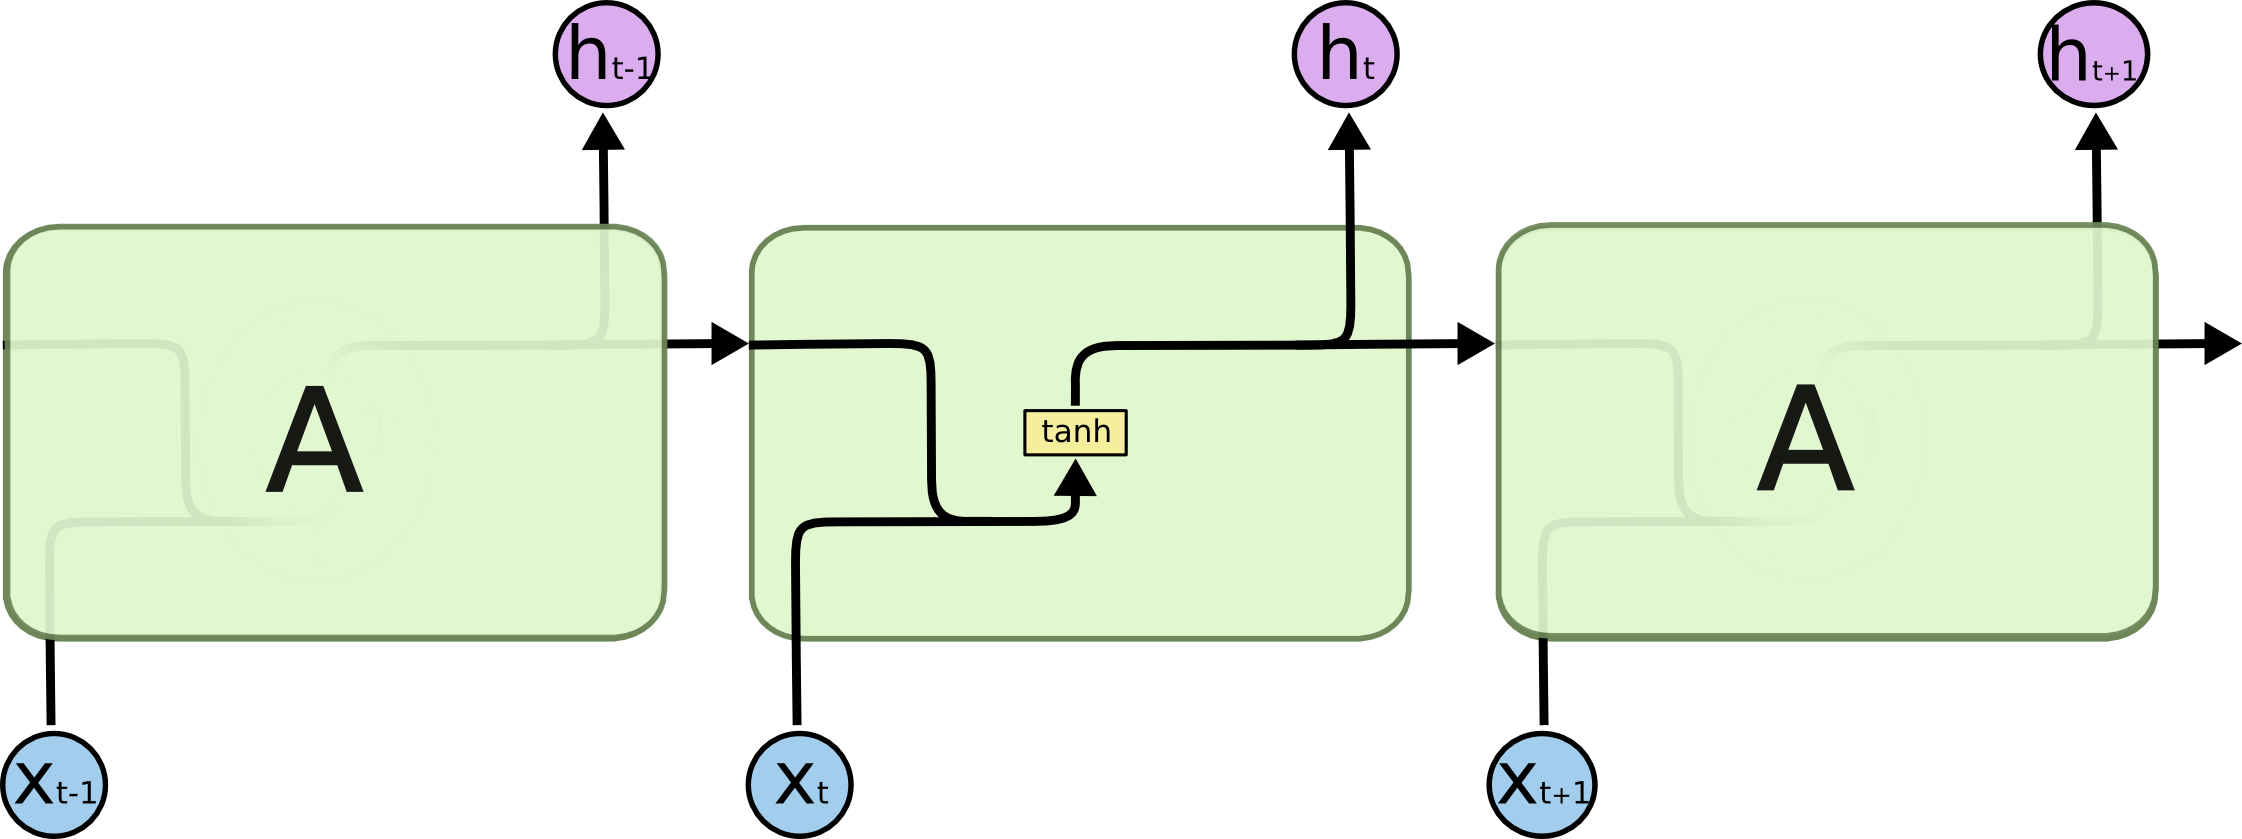
\includegraphics[width=\linewidth]{rnn_2.png}
	\caption{RNN unrolled standard. Nell'esempio viene usata la funzione di attivazione tangente iperbolica.}
	\label{fig:rnn_2}
\end{figure}
\begin{figure}[H]
	\centering
	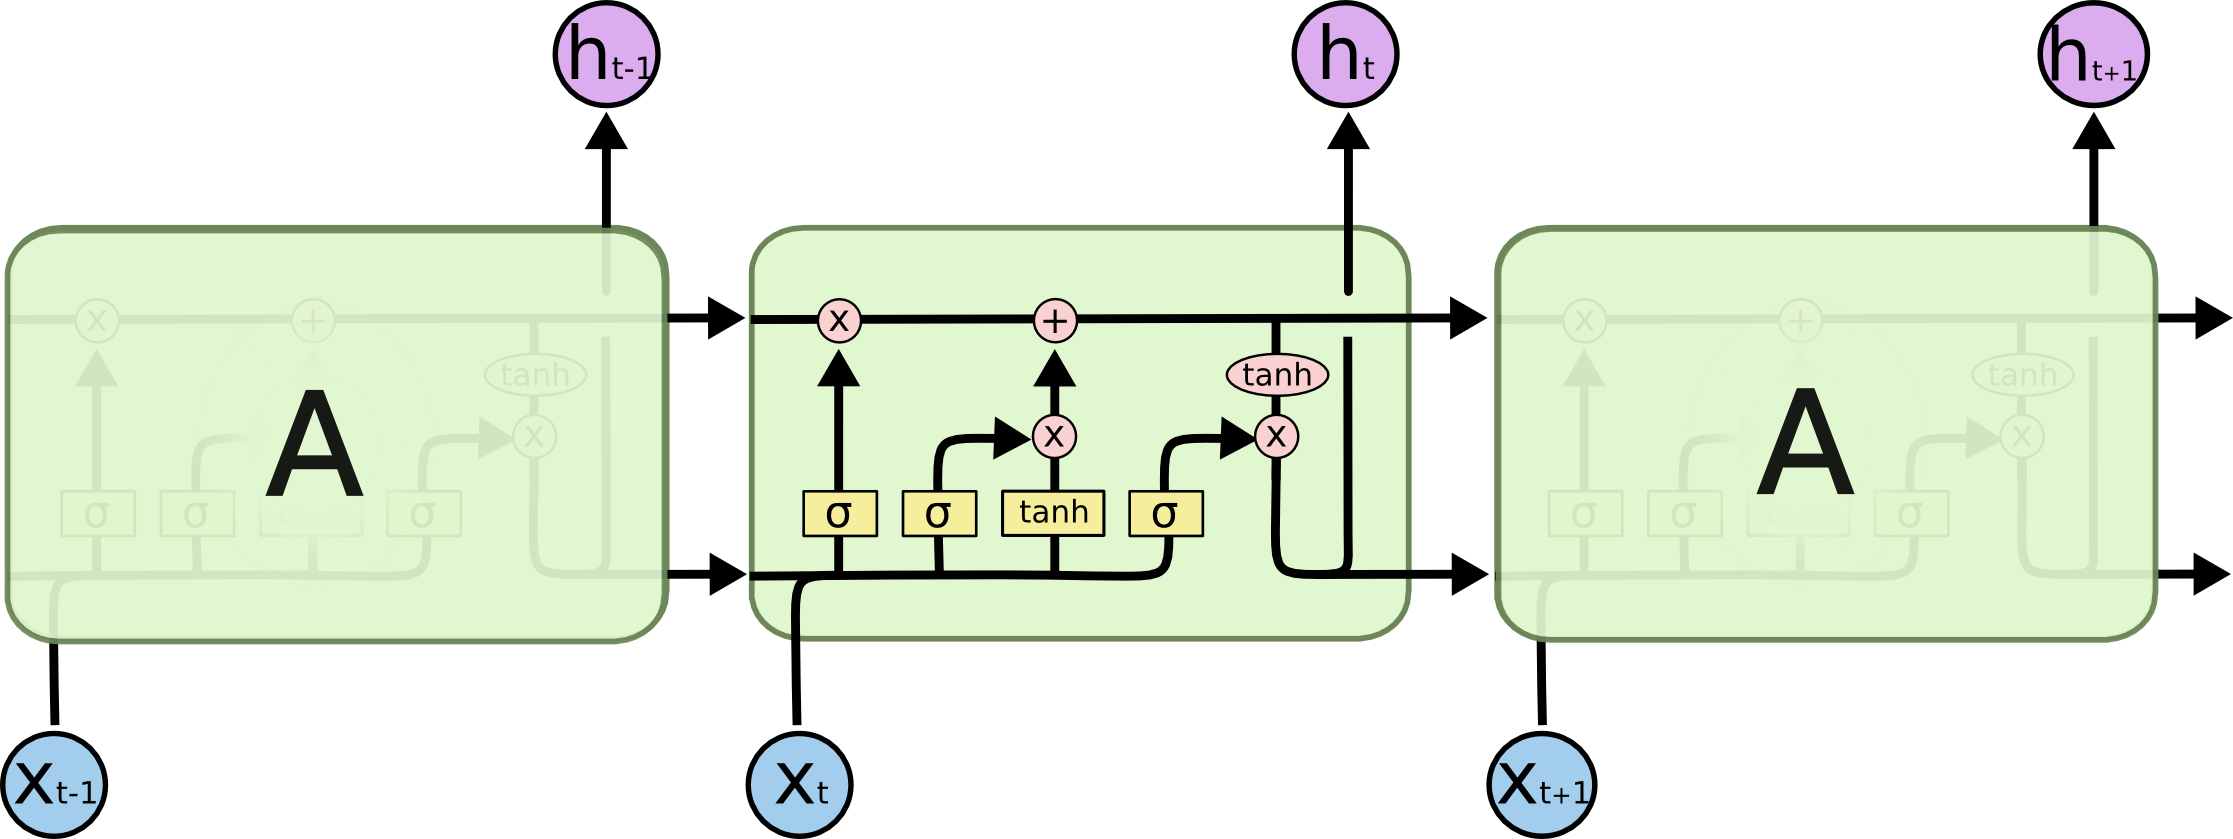
\includegraphics[width=\linewidth]{lstm.png}
	\caption{LSTM unrolled. I rettangoli gialli sono i quattro sotto-layer, di cui tre di essi applicano la semplice sigmoide, mentre l'altro la tangente iperbolica, mentre le figure rosa sono operazioni su vettori semplici.}
	\label{fig:lstm}
\end{figure}
La linea superiore della cella porta l'output superiore della cella precedente direttamente alla cella successiva, a meno di alcune operazioni lineari. Serve a mandare in avanti la conoscenza del passato senza modificarla troppo.\\
\\
La cella LSTM non segue necessariamente lo schema suddetto, ed esistono altre varianti, tutte accomunate dall'idea della linea superiore che preserva le long-term dependencies.\\
La \textbf{hidden size}, cioè dimensione dello stato nascosto, determina la dimensione dei quattro sotto-layer, ovvero il numero dei loro neuroni, quindi il numero totale dei neuroni presenti in una LSTM è dato dalla $hidden size * 4$. Tipicamente, al crescere della hidden size cresce anche la capacità di memorizzazione della LSTM.

\section{Autoencoder}
Un \textbf{autoencoder} è un rete neurale capace di apprendere caratteristiche da dati di training non etichettati, quindi in modo non supervisionato.\\
Un autoencoder prende i dati dall'input layer e li trasforma in una rappresentazione interna, detta \textbf{codifica} o \textbf{vettore latente}, da riusare per tentare di ricostruire l'input e mandarlo sull'output layer.\\
Lo scopo finale non è quello di ricostruire perfettamente l'input (sarebbe abbastanza inutile) ma quello di estrarre dagli input una codifica contenente le loro principali caratteristiche. In altre parole, si pone di cercare feature rilevanti nell'input.\\
\\
Per compiere la ricostruzione è necessario che input e output layer siano della stessa dimensione, tuttavia, al fine di permettere alla rete di estrarre le feature dagli input, il layer nascosto dove apparirà la codifica, detto \textbf{coding layer}, dovrà necessariamente essere di dimensione minore degli input e output layer. In questo caso si parla di autoencoder \textbf{undercomplete}.\\
Un autoencoder è sempre composto da due parti sostanzialmente:
\begin{itemize}
	\item Un \textbf{encoder}, una rete neurale che riduce l'input nella codifica. Anche detta \textit{rete ricognitica};
	\item Un \textbf{decoder}, una rete neurale che ricostruisce l'input dell'encoder a partire dalla codifica. Anche detta \textit{rete generativa};
\end{itemize}
Encoder e decoder sono simmetrici rispetto al coding layer.
\begin{figure}[H]
	\centering
	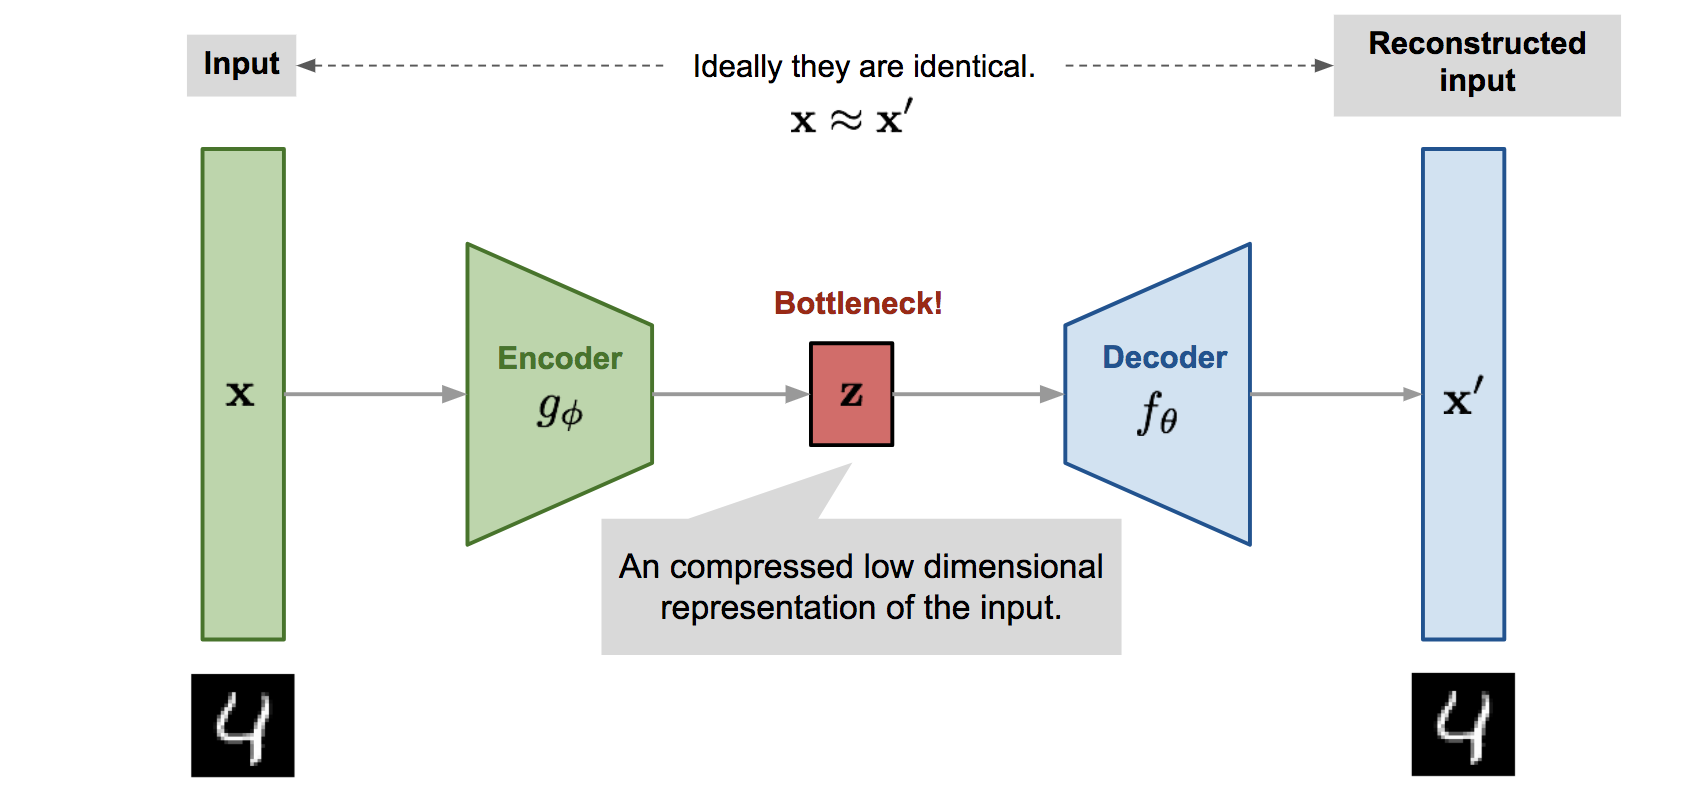
\includegraphics[width=\linewidth]{autoencoder.png}
	\caption{Schema di un autoencoder.}
	\label{fig:autoencoder}
\end{figure}
Gli autoencoder sono usati principalmente per fare \textbf{dimensionality reduction}, dato che la codifica è una rappresentazione ridotta di ogni input, ma anche \textbf{generazione di sample}, ovvero generare nuovi dati a partire da codifiche arbitrarie.\\
\\
Come una qualsiasi altra rete neurale, gli autoencoder possono essere resi più profondi aggiungendo layer nascosti, sia dal lato dell'encoder che dal lato del decoder. In tal caso si parla di \textbf{autoencoder stacked}.\\
In generale, un maggior livello di profondità permette alla rete di comprendere pattern più complessi, tuttavia una profondità troppo alta rende il rischio di overfitting più alto.


\section{Descrizione del modello proposto}
++++Perché lo abbiamo usato noi in questo caso
Struttura: stacked di LSTM insomma, sia per encoder che per decoder, e size coding layer
Come lo abbiamo usato (setting iperparametri, cosa abbiamo preso da esso (i vettori latenti) e cosa no)++++

\subsection{Training}
++++Come è stato allenato il modello (tensor flow e l'idea descritta con snippet notebook)++++

\section{Clustering con k-Means}
Per poter sfruttare la riduzione della dimensionalità compiuta dall'autoencoder, tutto il test set (di default corrispondente al 20\% del dataset) viene dato in input all'autoencoder per estrarne i relativi vettori latenti, ovvero la codifica delle TS di test.\\
Il k-Means viene lanciato cinque volte, seguendo questa regola. Sia n il numero di classi di un dataset:
\begin{enumerate}[(i)]
	\item Se $n\leq3$, allora si esegue da $2-$Means a $6-$Means;
	\item Se $n>2$, allora si esegue da $n-2-$Means ad $n+2-$Means.
\end{enumerate}
Ne viene lanciata l'implementazione di Scikit-Learn, retirata 100 volte (tramite il parametro $n\_init$) in modo tale che venga scelto il clustering migliore su 100 tentativi. Non viene fornito nessun random state in input.\\
Il k-Means usa come funzione di distanza quella euclidea, che risulta accettabile poiché i vettori latenti non sono delle TS, quindi la distanza DTW non è pienamente adatta, oltre che dispendiosa in termini di computazione.\\
\\
Per ciascuna esecuzione di k-Means viene mostrato il plot del clustering sui sample di test. Le metriche di valutazione, sia interne che esterne, sono tutte accumulate in un DataFrame di Pandas, esportato successivamente in CSV.

\subsection{Valutazione dei risultati}
Il modello presenta molti iperparametri, quindi il setting non è stato immediato. Si è ricordo alla \textbf{random search} per poter trovare una buona combinazione di iperparametri.\\
Per alcuni dataset, come ECG5000, ECG200, TwoLeadECG, PhalangesOutlineCorrect, ChlorineConcentration, questa ricerca ha portato miglioramenti in tutti gli score, mentre per gli altri dataset la ricerca non comportava alcun cambiamento sostanziale agli score.\\
Di seguito sono riportati i risultati del clustering dei dataset in esame dopo aver fatto il setting degli iperapametri:

\subsubsection{ECG5000}
\begin{center}
	\pgfplotstabletypeset[
	col sep=comma,
	string type,
	every head row/.style={
		before row={\hline
			\multicolumn{1}{c|}{\textbf{ECG5000}} &
			\multicolumn{2}{c|}{Internal} & \multicolumn{4}{c}{External} \\
		},
		after row=\hline
	},
	every last row/.style={after row=\hline},
	]{metrics/autoencoder/ECG5000_metrics.csv}
	\begin{table}[H]
		\centering
		\caption{k-Means sui vettori latenti del test set di ECG5000.}
	\end{table}
\end{center}

\subsubsection{ECG200}
\begin{center}
	\pgfplotstabletypeset[
	col sep=comma,
	string type,
	every head row/.style={
		before row={\hline
			\multicolumn{1}{c|}{\textbf{ECG200}} &
			\multicolumn{2}{c|}{Internal} & \multicolumn{4}{c}{External} \\
		},
		after row=\hline
	},
	every last row/.style={after row=\hline},
	]{metrics/autoencoder/ECG200_metrics.csv}
	\begin{table}[H]
		\centering
		\caption{k-Means sui vettori latenti del test set di ECG200.}
	\end{table}
\end{center}

\subsubsection{ChlorineConcentration}
\begin{center}
	\pgfplotstabletypeset[
	col sep=comma,
	string type,
	every head row/.style={
		before row={\hline
			\multicolumn{1}{c|}{\textbf{Chlorine}} &
			\multicolumn{2}{c|}{Internal} & \multicolumn{4}{c}{External} \\
		},
		after row=\hline
	},
	every last row/.style={after row=\hline},
	]{metrics/autoencoder/ChlorineConcentration_metrics.csv}
	\begin{table}[H]
		\centering
		\caption{k-Means sui vettori latenti del test set di ChlorineConcentration.}
	\end{table}
\end{center}

\subsubsection{FordA}
\begin{center}
	\pgfplotstabletypeset[
	col sep=comma,
	string type,
	every head row/.style={
		before row={\hline
			\multicolumn{1}{c|}{\textbf{FordA}} &
			\multicolumn{2}{c|}{Internal} & \multicolumn{4}{c}{External} \\
		},
		after row=\hline
	},
	every last row/.style={after row=\hline},
	]{metrics/autoencoder/FordA_metrics.csv}
	\begin{table}[H]
		\centering
		\caption{k-Means sui vettori latenti del test set di FordA.}
	\end{table}
\end{center}

\subsubsection{FordB}
\begin{center}
	\pgfplotstabletypeset[
	col sep=comma,
	string type,
	every head row/.style={
		before row={\hline
			\multicolumn{1}{c|}{\textbf{FordB}} &
			\multicolumn{2}{c|}{Internal} & \multicolumn{4}{c}{External} \\
		},
		after row=\hline
	},
	every last row/.style={after row=\hline},
	]{metrics/autoencoder/FordB_metrics.csv}
	\begin{table}[H]
		\centering
		\caption{k-Means sui vettori latenti del test set di FordB.}
	\end{table}
\end{center}

\subsubsection{PhalangesOutlinesCorrect}
\begin{center}
	\pgfplotstabletypeset[
	col sep=comma,
	string type,
	every head row/.style={
		before row={\hline
			\multicolumn{1}{c|}{\textbf{Phalanges}} &
			\multicolumn{2}{c|}{Internal} & \multicolumn{4}{c}{External} \\
		},
		after row=\hline
	},
	every last row/.style={after row=\hline},
	]{metrics/autoencoder/PhalangesOutlinesCorrect_metrics.csv}
	\begin{table}[H]
		\centering
		\caption{k-Means sui vettori latenti del test set di PhalangesOutlinesCorrect.}
	\end{table}
\end{center}

\subsubsection{RefrigerationDevices}
\begin{center}
	\pgfplotstabletypeset[
	col sep=comma,
	string type,
	every head row/.style={
		before row={\hline
			\multicolumn{1}{c|}{\textbf{Refrigeration}} &
			\multicolumn{2}{c|}{Internal} & \multicolumn{4}{c}{External} \\
		},
		after row=\hline
	},
	every last row/.style={after row=\hline},
	]{metrics/autoencoder/RefrigerationDevices_metrics.csv}
	\begin{table}[H]
		\centering
		\caption{k-Means sui vettori latenti del test set di RefrigerationDevices.}
	\end{table}
\end{center}

\subsubsection{TwoLeadECG}
\begin{center}
	\pgfplotstabletypeset[
	col sep=comma,
	string type,
	every head row/.style={
		before row={\hline
			\multicolumn{1}{c|}{\textbf{TwoLeadECG}} &
			\multicolumn{2}{c|}{Internal} & \multicolumn{4}{c}{External} \\
		},
		after row=\hline
	},
	every last row/.style={after row=\hline},
	]{metrics/autoencoder/TwoLeadECG_metrics.csv}
	\begin{table}[H]
		\centering
		\caption{k-Means sui vettori latenti del test set di TwoLeadECG.}
	\end{table}
\end{center}

\subsubsection{TwoPatterns}
\begin{center}
	\pgfplotstabletypeset[
	col sep=comma,
	string type,
	every head row/.style={
		before row={\hline
			\multicolumn{1}{c|}{\textbf{TwoPatterns}} &
			\multicolumn{2}{c|}{Internal} & \multicolumn{4}{c}{External} \\
		},
		after row=\hline
	},
	every last row/.style={after row=\hline},
	]{metrics/autoencoder/TwoPatterns_metrics.csv}
	\begin{table}[H]
		\centering
		\caption{k-Means sui vettori latenti del test set di TwoPatterns.}
	\end{table}
\end{center}

Da questi risultati è possibile fare una serie di osservazioni sulle misure:
\begin{enumerate}
	\item Le \textbf{misure interne sono molto influenzate dal numero di cluster}, andando a peggiorare man mano che il numero cresce.\\
	Questo, chiaramente, dipende molto dalla disposizione dei dati nello spazio e anche dal tipo di algoritmo di clustering: k-Means, infatti, non ottimizza la densità dei cluster, a differenza di altri come DBSCAN;
	\item Le \textbf{misure esterne sono molto suscettibili con piccoli dataset}, infatti, nel caso di ECG200, si hanno ARI ed FMI abbastanza bassi.\\
	Il motivo risiede nel fatto che le metriche esterne sono basate su conteggi non pesati;
	\item Le misure di \textbf{purity e relative purity sono abbastanza indipendenti dal numero di cluster}.\\
	Questo potrebbe significare che sono più influenzare dalla natura del dataset e dalle caratteristiche che l'autoencoder è stato in grado di estrarre, piuttosto che dal numero di cluster.
\end{enumerate}

Inoltre, è stato possibile fare le seguenti osservazioni sul modello e sui dataset:
\begin{enumerate}	
	\item Nei \textbf{dataset degli elettrocardiogrammi le misure esterne sono tendenzialmente alte}. Questo significa che l'autoencoder è riuscito a estrarre quelle caratteristiche che gli autori dei dataset hanno usato per fare il labelling degli elettrocardiogrammi.\\
	Questo non accade per gli altri dataset, o almeno non con gli stessi score;
	\item \textbf{Le caratteristiche delle TS molto "rumorose"}\footnote{hanno dei pattern che continuamente alternano valori alti e valori bassi} \textbf{non riescono ad essere estratte bene dall'autoencoder}, e questo si rispecchia nelle misure interne basse e nelle misure esterne che ricordano quelle del random labelling. Questo accade per FordA, FordB, RefrigerationDevices e TwoPatterns;
\end{enumerate}